\documentclass[serif,final,bigger]{beamer}
\usepackage{enumerate}
\usepackage{graphicx}
\usepackage{svg}

\usetheme{Rochester}
\usecolortheme{beaver}
\linespread{1.6}  % Double spacing
\graphicspath{{../figures/}}

\title{Forecasting Lost Person Survival}
\author{Jonathan Lee}
\institute{TJHSST Computer Systems Lab}
\date{June 2, 2016}

\begin{document}
  \usebackgroundtemplate{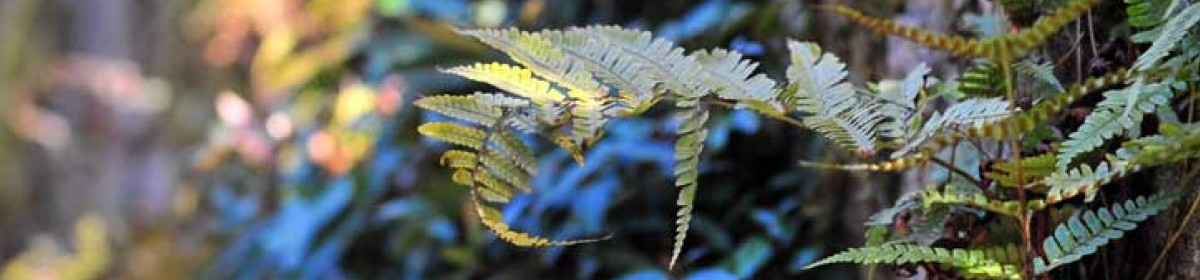
\includegraphics[width=\paperwidth]{ferns}}
  \begin{frame}
    \titlepage
  \end{frame}
  \usebackgroundtemplate{}

  \section{Introduction}

  \begin{frame}
    \frametitle{Purpose}
    \begin{itemize}
      \item Advise wilderness search-and-rescue (WiSAR) personnel when to terminate a search
      \item Augment lost person motion models
    \end{itemize}
  \end{frame}

  \begin{frame}
    \frametitle{Goals}
    \begin{itemize}
      \item Classify subjects as alive or dead-on-arrival (DOA)
      \item Describe a subject's probability of survival over time
    \end{itemize}
  \end{frame}

  \section{Methods}

  \begin{frame}
    \frametitle{Data Preparation}
    \begin{itemize}
      \item International Search \& Rescue Incident Database (ISRID)
      \item Cleaning and validation
      \item SQLAlchemy backend
      \item Unit testing
      \item External historic weather data API
    \end{itemize}
  \end{frame}

  \begin{frame}
    \frametitle{Survival Function}
    $$S(t) = P(T > t) = 1 - F_T(t) = \int_t^\infty f_T(u) du$$
    $$S(0) = 1, \lim_{t \to \infty} S(t) = 0$$
  \end{frame}

  \begin{frame}
    \frametitle{Kaplan-Meier}
    \begin{itemize}
      \item Empirical, stepwise, decreasing survival over time (non-parametric)
      $$S(t) = \prod_{t_i < t} \frac{n_i - d_i}{n_i}$$
      \item Curve should approach the true survival function
      \item Handles right-censoring
    \end{itemize}
  \end{frame}

  \begin{frame}
    \frametitle{Evaluation}
    \begin{itemize}
      \item Brier Score
      $$0 \leq \frac{1}{N} \sum_{i=1}^N (y_i - o_i)^2 \leq 1$$
    \end{itemize}
  \end{frame}

  \section{Results}

  \setsvg{svgpath = ../figures/kaplan-meier/}

  \begin{frame}
    \frametitle{Kaplan-Meier Plots}
    \includesvg[width=\textwidth]{km-single-grid-large}
  \end{frame}

  \begin{frame}
    \frametitle{Kaplan-Meier Plots}
    \includesvg[width=\textwidth]{km-single-combined-large}
  \end{frame}

  \section{Conclusion}

  \begin{frame}
    \frametitle{Future Work}
  \end{frame}

  \section{Appendix}

  \begin{frame}
    \frametitle{References}
  \end{frame}
\end{document}
